% This is LLNCS.DEM the demonstration file of
% the LaTeX macro package from Springer-Verlag
% for Lecture Notes in Computer Science,
% version 2.4 for LaTeX2e as of 16. April 2010
%
\documentclass{llncs}
\usepackage{graphicx}
\usepackage{hyperref}
\usepackage[spanish]{babel}
%
\usepackage{makeidx}  % allows for indexgeneration
%
\begin{document}
%
\frontmatter          % for the preliminaries
%
\pagestyle{headings}  % switches on printing of running heads
%\addtocmark{Hamiltonian Mechanics} % additional mark in the TOC
%
%\chapter*{Preface}
%
%This textbook is intended for use by students of physics, physical
%chemistry, and theoretical chemistry. The reader is presumed to have a
%basic knowledge of atomic and quantum physics at the level provided, for
%example, by the first few chapters in our book {\it The Physics of Atoms
%and Quanta}. The student of physics will find here material which should
%be included in the basic education of every physicist. This book should
%furthermore allow students to acquire an appreciation of the breadth and
%variety within the field of molecular physics and its future as a
%fascinating area of research.
%
%For the student of chemistry, the concepts introduced in this book will
%provide a theoretical framework for that entire field of study. With the
%help of these concepts, it is at least in principle possible to reduce
%the enormous body of empirical chemical knowledge to a few basic
%principles: those of quantum mechanics. In addition, modern physical
%methods whose fundamentals are introduced here are becoming increasingly
%important in chemistry and now represent indispensable tools for the
%chemist. As examples, we might mention the structural analysis of
%complex organic compounds, spectroscopic investigation of very rapid
%reaction processes or, as a practical application, the remote detection
%of pollutants in the air.

%\vspace{1cm}
%\begin{flushright}\noindent
%April 1995\hfill Walter Olthoff\\
%Program Chair\\
%ECOOP'95
%\end{flushright}
%%
%\chapter*{Organization}
%ECOOP'95 is organized by the department of Computer Science, Univeristy
%of \AA rhus and AITO (association Internationa pour les Technologie
%Object) in cooperation with ACM/SIGPLAN.
%%
%\section*{Executive Commitee}
%\begin{tabular}{@{}p{5cm}@{}p{7.2cm}@{}}
%Conference Chair:&Ole Lehrmann Madsen (\AA rhus University, DK)\\
%Program Chair:   &Walter Olthoff (DFKI GmbH, Germany)\\
%Organizing Chair:&J\o rgen Lindskov Knudsen (\AA rhus University, DK)\\
%Tutorials:&Birger M\o ller-Pedersen\hfil\break
%(Norwegian Computing Center, Norway)\\
%Workshops:&Eric Jul (University of Kopenhagen, Denmark)\\
%Panels:&Boris Magnusson (Lund University, Sweden)\\
%Exhibition:&Elmer Sandvad (\AA rhus University, DK)\\
%Demonstrations:&Kurt N\o rdmark (\AA rhus University, DK)
%\end{tabular}
%%
%\section*{Program Commitee}
%\begin{tabular}{@{}p{5cm}@{}p{7.2cm}@{}}
%Conference Chair:&Ole Lehrmann Madsen (\AA rhus University, DK)\\
%Program Chair:   &Walter Olthoff (DFKI GmbH, Germany)\\
%Organizing Chair:&J\o rgen Lindskov Knudsen (\AA rhus University, DK)\\
%Tutorials:&Birger M\o ller-Pedersen\hfil\break
%(Norwegian Computing Center, Norway)\\
%Workshops:&Eric Jul (University of Kopenhagen, Denmark)\\
%Panels:&Boris Magnusson (Lund University, Sweden)\\
%Exhibition:&Elmer Sandvad (\AA rhus University, DK)\\
%Demonstrations:&Kurt N\o rdmark (\AA rhus University, DK)
%\end{tabular}
%%
%\begin{multicols}{3}[\section*{Referees}]
%V.~Andreev\\
%B\"arwolff\\
%E.~Barrelet\\
%H.P.~Beck\\
%G.~Bernardi\\
%E.~Binder\\
%P.C.~Bosetti\\
%Braunschweig\\
%F.W.~B\"usser\\
%T.~Carli\\
%A.B.~Clegg\\
%G.~Cozzika\\
%S.~Dagoret\\
%Del~Buono\\
%P.~Dingus\\
%H.~Duhm\\
%J.~Ebert\\
%S.~Eichenberger\\
%R.J.~Ellison\\
%Feltesse\\
%W.~Flauger\\
%A.~Fomenko\\
%G.~Franke\\
%J.~Garvey\\
%M.~Gennis\\
%L.~Goerlich\\
%P.~Goritchev\\
%H.~Greif\\
%E.M.~Hanlon\\
%R.~Haydar\\
%R.C.W.~Henderso\\
%P.~Hill\\
%H.~Hufnagel\\
%A.~Jacholkowska\\
%Johannsen\\
%S.~Kasarian\\
%I.R.~Kenyon\\
%C.~Kleinwort\\
%T.~K\"ohler\\
%S.D.~Kolya\\
%P.~Kostka\\
%U.~Kr\"uger\\
%J.~Kurzh\"ofer\\
%M.P.J.~Landon\\
%A.~Lebedev\\
%Ch.~Ley\\
%F.~Linsel\\
%H.~Lohmand\\
%Martin\\
%S.~Masson\\
%K.~Meier\\
%C.A.~Meyer\\
%S.~Mikocki\\
%J.V.~Morris\\
%B.~Naroska\\
%Nguyen\\
%U.~Obrock\\
%G.D.~Patel\\
%Ch.~Pichler\\
%S.~Prell\\
%F.~Raupach\\
%V.~Riech\\
%P.~Robmann\\
%N.~Sahlmann\\
%P.~Schleper\\
%Sch\"oning\\
%B.~Schwab\\
%A.~Semenov\\
%G.~Siegmon\\
%J.R.~Smith\\
%M.~Steenbock\\
%U.~Straumann\\
%C.~Thiebaux\\
%P.~Van~Esch\\
%from Yerevan Ph\\
%L.R.~West\\
%G.-G.~Winter\\
%T.P.~Yiou\\
%M.~Zimmer\end{multicols}
%
%\section*{Sponsoring Institutions}
%
%Bernauer-Budiman Inc., Reading, Mass.\\
%The Hofmann-International Company, San Louis Obispo, Cal.\\
%Kramer Industries, Heidelberg, Germany
%
%\tableofcontents
%
\mainmatter              % start of the contributions
%
\title{ Diseño, Implementación,
	Evaluación y Análisis de Sistemas de Recuperación de Información}
%
%\titlerunning{Hamiltonian Mechanics}  % abbreviated title (for running head)
%                                     also used for the TOC unless
%                                     \toctitle is used
%
\author{Dayany Alfaro González \and Dalianys Pérez Perera}
%
%\authorrunning{Ivar Ekeland et al.} % abbreviated author list (for running head)
%
%%%% list of authors for the TOC (use if author list has to be modified)
%\tocauthor{Ivar Ekeland, Roger Temam, Jeffrey Dean, David Grove,
%Craig Chambers, Kim B. Bruce, and Elisa Bertino}
%
\institute{Universidad de La Habana, San Lázaro y L, Plaza de la Revolución, La Habana, Cuba%,\\
%\email{I.Ekeland@princeton.edu},\\ WWW home page:
%\texttt{http://users/\homedir iekeland/web/welcome.html
}
%\and
%Universit\'{e} de Paris-Sud,
%Laboratoire d'Analyse Num\'{e}rique, B\^{a}timent 425,\\
%F-91405 Orsay Cedex, France}

\maketitle              % typeset the title of the contribution

\begin{abstract}
La Recuperación de Información (RI) es la ciencia que permite el almacenamiento y rápido acceso a gran cantidad de información. Machine Learning juega un importante rol en muchos aspectos en los sistemas de RI modernos. Este trabajo presenta los resultados de una profunda investigación realizada sobre el potencial de las Redes Neuronales en este tema. Inicialmente se propone una versión de modelo vectorial utilizando herramientas avanzadas en procesamiento de lenguaje natural y también dos enfoques diferentes de modelos neuronales que hacen uso de redes Long-Short Term Memory (LSTM) y Convolutional Neural Networks(CNN).

\keywords{Recuperación de Información, Modelo Vectorial de Recuperación de Información, Modelo Neuronal de Recuperación de Información, LSTM , MatchPyramid}

\end{abstract}
%
\section{Introducción}
%
La Recuperación de Información (RI) es un campo de la informática que permite a un sistema de RI (SRI) seleccionar, de una colección de documentos, aquellos que probablemente correspondan a la necesidad de información de un usuario. Más específicamente, la RI es principalmente la actividad de obtener recursos de información, como documentos o respuestas, que se supone que coinciden con una necesidad expresada como una consulta o una pregunta.

Los modelos de RI se proponen e implementan para hacer frente al objetivo principal de RI, recuperar información relevante para una consulta. La mayoría de los modelos de RI se basan en el mismo supuesto, los documentos y consultas se representan como Bag-of-Words(BoW) o bolsa de palabras en español y la relevancia se interpreta de la misma forma que la coincidencia léxica entre palabras de consulta y palabras de documento. Estos modelos estiman el ranking de relevancia basándose en la coincidencia exacta entre las palabras de las secuencias de texto de entrada. Por lo tanto, algunos documentos devueltos por el SRI no siempre satisfacen la intención del usuario con la consulta. Esta limitación se debe a las representaciones de BoW, las cuales consideran cada secuencia de texto como un conjunto de palabras independientes. El problema principal resultado de estos enfoques es el desajuste de vocabulario. Este consiste en usar un vocabulario diferente en la consulta y sus correspondientes relevantes resultados (documentos).

Nuestra propuesta inicial fue una aproximación de un modelo Vectorial, auxiliándonos de herramientas avanzadas para el procesamiento de texto y la representación vectorial de las sentencias mediante diferentes pesos. Este acercamiento no proporcionó buenos resultados por lo que se decidió guiar la investigación hacia otras lineas de estudio. En los últimos años se han dedicado grandes esfuerzos al intento de mejorar el rendimiento de los sistemas de RI y la investigación ha explorado muchas direcciones diferentes tratando de utilizar los provechosos resultados obtenidos en otras áreas. En este trabajo investigaremos la posibilidad de utilizar Redes Neuronales en RI. 

Los modelos neuronales aprenden representaciones del lenguaje a partir del texto procesado lo cual puede salvar la brecha entre el vocabulario de consultas y documentos. Una consulta, normalmente contiene poca cantidad de términos, mientras que la longitud de los documentos, dependiendo del escenario, puede variar desde unos pocos términos hasta cientos de oraciones o más. Los modelos para RI utilizan representaciones vectoriales de texto y, por lo general, contienen una gran cantidad de parámetros que necesitan ser ajustados. El aprendizaje de representaciones adecuadas de texto también exige conjuntos de datos a gran escala para el entrenamiento. Por lo tanto, a diferencia de los modelos de RI clásicos, estos enfoques neuronales tienden a consumir datos, con un rendimiento que mejora con más datos de entrenamientos.

Impulsado por los avances que ha tenido el aprendizaje profundo en investigaciones de visión por computadora, las redes neuronales han resurgido como un paradigma popular de aprendizaje de máquina en muchas otras direcciones de investigación, incluida la recuperación de información. Uno de nuestros modelos pretende extraer las características semánticas de las sentencias a través de redes neuronales recurrentes, específicamente 2 redes LSTM, una para codificar la consulta y otra para el documento. Las componentes principales son los embeddings a nivel de palabras utilizados, los vectores de sentencia y el comparador inmerso en el modelo. Otro de los modelos hará uso principalmente de una matriz de \textit{matching} entre la consulta y el documento, la cual será procesada por una Red Convolucional (CNN) con el objetivo de extraer patrones que resulten útiles para determinar similaridad. La implementación se llevó a cabo usando el lenguaje de programación Python y en específico, para los modelos neuronales usamos el framework \texttt{keras} con \texttt{tensorflow} como backend.   
%
\section{Trabajos Relacionados}
%
Las redes neuronales son conocidas por su capacidad de construir, en un espacio latente, representaciones que son capaces de capturar la semántica de diferentes tipos de información (por ejemplo, imágenes, sonido, texto). En los últimos años, las redes neuronales profundas han llegado a un progreso notable en varias áreas de investigación, como el reconocimiento del habla, visión por computadora y minería de texto, incluidas varias tareas de IR \cite{11}. En el procesamiento de texto, los modelos neuronales se utilizan para construir representaciones ditribuidas(embeddings) de palabras y secuencias, así como para realizar el proceso de matching.

Machine learning (ML) ha sido empleado en tareas de RI desde la década de 1980 \cite{206}. En este sentido, dichos algoritmos son usados en dos objetivos principales: (1) para aprendizaje de representaciones textuales \cite{12}\cite{55}, donde la representación de la entrada es optimizada durante el entrenamiento, y (2) para matching \cite{185,207}, donde es aprendida una función de ranking. La mayoría de los modelos de RI están dirigidos al aprendizaje de funciones de ranking \cite{205,208,209,210,211} y son referenciados como modelos Learning to Rank(LTR). Todos los métodos LTR pueden ser agrupados \cite{207} en 3 enfoques: \textit{pointwise}, \textit{pairwise} y \textit{listwise}, los cuales difieren en cuanto al objetivo a aprender. 

Los diferentes modelos neuronales para aplicaciones de \textit{text matching} se dividen en dos grupos principales \cite{178}, específicamente los modelos centrados en la representación de la información y los modelos enfocados en la interacción. Los de la primera clase intentan aprender patrones latentes que mejor representan las secuencias de entrada, a continuación se mencionan algunos de ellos.

Huang et al \cite{16} propone un Deep Structured Semantic Model (DSSM) para búsqueda web ad-hoc. La entrada consiste en dos ramas simétricas profundas, una para la consulta y otra para el documento. El espacio de embedding contiene un conjunto de representaciones de vectores aprendidos a nivel de letras. La representación intermedia constituye la concatenación de diferentes vectores de \textit{n}-gramas de las secuencias de entrada. La capa de \textit{matching} la sustituye la función de similitud del coseno. El trabajo de Shen et al \cite{237} extiende el modelo DSSM introduciendo una red neuronal convolucional (CNN) en la arquitectura.

En otros modelos, la función de representación podría ser una CNN de múltiples capas de convolución y agrupación, como en el modelo LTR convolucional de Severyn y Moschitti \cite{238} y el modelo ARC-I de HU et al. \cite{17}. Por ejemplo el modelo LTR convolucional \cite{238} primero concatena cada vector de palabras y calcula la representación correspondiente de cada secuencia mediante una capa CNN. En la parte de \textit{matching} es utilizada una matriz de similaridad $M$.

El modelo MV-LSTM de Wan et al. \cite{3} utiliza capas BiLSTM para aprender representaciones basadas en determinadas posiciones para cada secuencia de entrada. Algunos modelos recurrentes \cite{243,241} combinan señales de representación calculadas por los estados ocultos de las redes recurrentes, con señales externas para fortalecer las representaciones finales.

Con respecto a los modelos centrados en la interacción, intentan aprender diferentes características de similaridad dadas las representaciones distribuidas iniciales de las secuencias de entrada. La función de \textit{matching} puede ser definida mediante una matriz $M$ la cual representa \textit{matchings} a nivel de palabras, su formulación varía en los diferentes modelos del estado del arte. 

\section{Representación semántica}

Las representaciones distribuidas son las que tienen en cuenta el contexto de ocurrencia de la palabra. Se conocen popularmente como word embeddings. Estas condensan la información de la palabra y su contexto en un número menor de dimensiones y con información de su significado.

La representación semántica distribuida conocida como Word2Vec, constituye un medio para encapsular las apariciones de palabras en texto como elementos en un espacio vectorial \cite{2}. Este método es bastante exitoso, pero por su naturaleza, crea embeddings para palabras sueltas (y frases cortas comunes) solamente. La universidad de Stanford desarrolló otro método para computar la semántica distribuida de las palabras, y este método se conoce como GloVe. GloVe es similar a Word2Vec, calcula la frecuencia de ocurrencia de cada palabra y crea un vector de una dimensión específica para representar una palabra, pero los métodos que utilizan son más basados en álgebra lineal \cite{0}. En esta investigación se usaron los embeddings \texttt{glove-wiki-gigaword-50} y \texttt{glove-wiki-gigaword-300} con vectores de dimensión 50 y 300 respectivamente.

Se han desarrollado varios métodos para obtener el embedding de una oración representada por una secuencia de palabras, cada una con su propio vector. Algunos de estos métodos implican el uso de redes neuronales como por ejemplo LSTM y sus variaciones. (Arora et al. 2016) \cite{1} propuso un baseline para embeddings de oraciones llamado método SIF el cual implica tomar el promedio de todos los vectores de palabras en una oración y eliminar la primera componente. 

\section{Sistemas de Recuperación de Información Propuestos}


\subsection{Procesamiento de los Datos}

En todas las propuestas se procesan los datos de la misma forma. Los corpus utilizados para los experimientos se pueden descargar aquí \href{http://ir.dcs.gla.ac.uk/resources/test_collections/} {http://ir.dcs. gla.ac.uk/resources/test\_collections/}, sus nombres son CISI, Cranfield y Medline. Estos mantienen formatos similares, lo cual facilitó el \textit{parsing} de los mismos.

A cada sentencia(documentos y consultas) extraída se le aplicó un preprocesamiento para obtener una representación vectorial que capturara mayores características semánticas. Primeramente, se separa la oración en tokens utilizando el módulo \texttt{wordpunct\_tokenize} de nltk( Natural Language ToolKIt), eliminando signos de puntuación y espacios en blanco. Luego son descartados los stopwords que se encuentran en \texttt{nltk.corpus.stopwords} y removidos los sufijos detectados. En esta última fase de stemming se empleó PorterStemmer, perteneciente a la librería \texttt{gensim}, específicamente \texttt{gensim.parsing.porter}. Finalmente, cada sentencia constituye una lista de términos que serán comparadas utilizando algoritmos de similaridad.

\subsection{Modelo Vectorial}

Esta propuesta se apoya en gran medida de herramientas ya implementadas para representar vectorialmente el conjunto de documentos ya procesado. Una vez tenido preprocesada cada sentencia se construye un diccionario donde las llaves constituyen el conjunto de palabras presentes y los valores serían el identificador (id) correspondiente a cada una. A partir de este diccionario, se convierte a cada documento en una lista de tuplas de la forma (token\_id, token\_count), o sea, en la clásica representación BoW, que es un enfoque común utilizado para representar texto en tareas de recuperación de información en particular. Posee una estructura simple sin capturar conocimientos lingúísticos ni de contexto.

De la unión de las listas anteriores se obtiene lo que sería el corpus representativo del dataset en cuestión. 
El mismo encapsula los valores de frecuencia de las palabras y conforma la entrada a los modelos mencionados. En este trabajo se emplearon 4 modelos que se encuentran en la librería \texttt{gensim.models}. A continuación se muestra una breve descripción de los mismos:
\begin{itemize}
	\item \textbf{TdidfModel}: transforma una matriz de ocurrencia de términos en una matriz con el esquema clásico TF(term frequency)-IDT(inverse document frequency)
	\item \textbf{LsiModels}(Latent Semantic Indexing): Implementa SVD(Singular Value Decomposition). La descomposición de SVD se puede actualizar con nuevas observaciones en cualquier momento, para un entrenamiento en línea, incremental y eficiente en la memoria. Permite identificar patrones y relaciones entre términos y temas. 
	\item \textbf{LdaModel}(Latent Dirichlet Allocation): Este módulo permite tanto la estimación del modelo LDA a partir de un corpus de capacitación, como la inferencia de la distribución de temas en documentos nuevos y no vistos. El modelo también se puede actualizar con nuevos documentos.
	\item \textbf{LogEntropyModel}: Este módulo permite transformar un corpus simple representado con Bag of Words (BoW) en un espacio de entropía logarítmico. Produce una representación de frecuencia de términos con pesos logarítmicos.
	
\end{itemize}

	En esencia cada modelo representa de forma diferente la información semántica contenida en el corpus y es muy útil para obtener dicha representación en las nuevas consultas generadas. Transforman un vector de un espacio hacia otro.
	
Finalmente es necesario evaluar la similaridad entre el conjunto de documentos y una consulta. Para ello se usó la matriz de similaridad de \texttt{gensim}, MatrixSimilarity. Esta matriz recibe el corpus y devuelve un ranking entre todos los documentos respecto a la consulta, utilizando la métrica del coseno. En la Figura \ref{vect} se muestra cómo quedaría conformado un pipeline completo de estos modelos.


\begin{figure}
	\begin{center}
		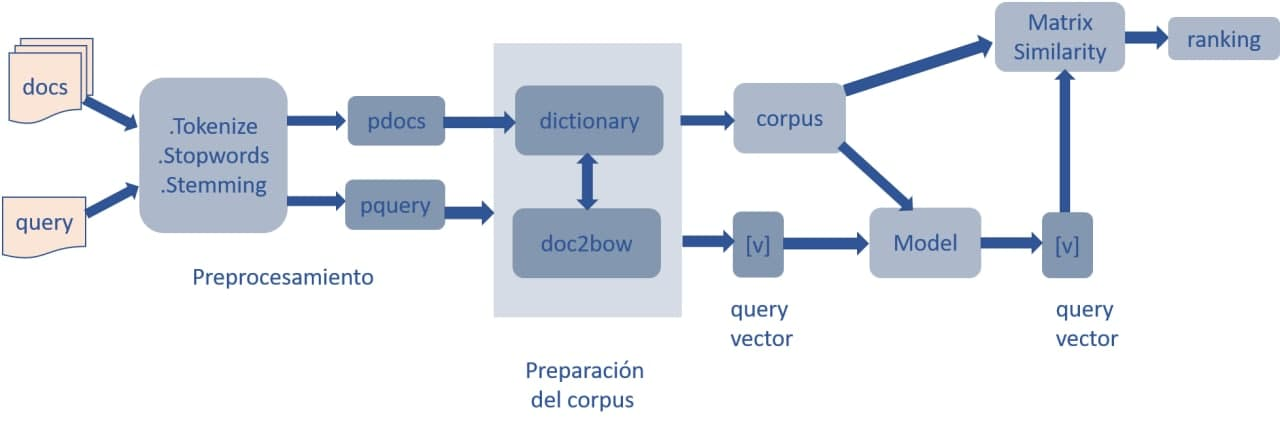
\includegraphics[width=\linewidth]{ ./images/vect.jpg}
		\caption{Esquema de la versión de modelo vectorial.}
		\label{vect}
	\end{center}
\end{figure}


\subsubsection{Evaluación.} 
En las Tablas \ref{medline}, \ref{cisi}, \ref{cran} se muestran los valores obtenidos de promediar la precisión y el recobrado obtenidos al aplicar cada uno de los modelos a las colecciones de prueba seleccionadas. Como se puede observar, los resultados para nada son buenos, con muy bajos niveles de precisión y recobrado. El modelo TdidfModel arrojó mejores valores de estas métricas en los tres datasets empleados. En general son mejores los resultados en el dataset Medline lo cual puede deberse a la dimensión del dataset, teniendo menor cantidad de documentos y consultas.

\begin{table}
	\caption{Dataset: Medline (documentos: 1033 consultas: 30)}
	\label{medline} 
	\begin{tabular}{|l|c|c|c|c|}
		\hline
		\textbf{Métrica} & \textbf{TdidfModel} & \textbf{LsiModels} & \textbf{LdaModel} &  \textbf{LogEntropyModel} \\
		\hline
		Precisión & 0.25590 & 0.02000 & 0.02014 & 0.25924 \\
		\hline
		Recobrado & 0.51909 & 0.03823 & 0.03919 & 0.52436 \\
		\hline
	\end{tabular} 
\end{table}

\begin{table}
	\caption{Dataset: CISI (documentos: 1460 consultas: 112)}
	\label{cisi}
	\begin{tabular}{|l|c|c|c|c|}
		\hline
		\textbf{Métrica} & \textbf{TdidfModel} & \textbf{LsiModels} & \textbf{LdaModel} &  \textbf{LogEntropyModel} \\
		\hline		
		Precisión & 0.03607 & 0.00955 & 0.00604 & 0.00910 \\
		\hline
		Recobrado & 0.05030 & 0.01641 & 0.00665 & 0.01213 \\
		\hline
	\end{tabular} 
\end{table}

\begin{table}
	\caption{Dataset: Cranfield (documentos: 1400 consultas: 225)}
	\label{cran}
	\begin{tabular}{|l|c|c|c|c|}
		\hline
		\textbf{Métrica} & \textbf{TdidfModel} & \textbf{LsiModels} & \textbf{LdaModel} &  \textbf{LogEntropyModel} \\
		\hline
		Precisión & 0.04284 & 0.00248 & 0.00201 & 0.01062 \\
		\hline
		Recobrado & 0.27418 & 0.01535 & 0.01319 & 0.06776 \\
		\hline
	\end{tabular} 
\end{table}

\subsection{Modelo Neuronal con Redes LSTM}

Nuestra segunda propuesta estuvo motivada por el éxito de las redes Long-Short Term Memory (LSTM) en tareas de procesamiento de lenguaje natural como traducción automática, clasificación de textos, chatbots, debido a su capacidad de aprender dependencias entre términos a largo plazo. El modelo LSTM es construido a partir del modelo RNN básico, evitando una de las limitaciones de estas últimas al trabajar con largas secuencias, conocido como \textit{vanishing gradient problem}. 
LSTM desarrolla una celda de memoria y usa filtros para decidir cuánta información debe olvidarse o debe fluir a través de los pasos de tiempo. De esta manera, se puede guardar información útil y se puede descartar información innecesaria. El modelo LSTM y sus variantes como Gated Recurrent Unit (GRU) han demostrado que si se entrena de manera efectiva puede codificar el significado de las oraciones en representaciones vectoriales de longitud fija. 

\subsubsection{Representación de las Sentencias.}

El modelo recibe como entrada dos sentencias que constituyen listas de términos ya preprocesadas pero es necesario obtener una representación vectorial de las mismas. Para ello se emplearon los embeddings de palabras. Estos mecanismos permiten asignar un vector de determinado espacio a cada palabra, de forma tal que a dos palabras semánticamente equivalentes les correspondan vectores lo más cercanos posible en dicho espacio. Para cada dataset se salvó un diccionario con los vectores asociados a cada palabra, evitando así recalcular estos valores de una corrida a otra. En este trabajo se empleó en la mayoría de los experimentos el embedding preentrenado g\texttt{love-wiki-gigaword-50}. 

Luego cada sentencia quedaría conformada por la unión de los vectores correspondientes a cada uno de sus términos. Por ejemplo la sentencia $s_1 = [w_1, w_2, w_3, ..., w_t]$ se representa vectorialmente como un vector donde cada componente tiene dimensión 50 $s1 = [WE(w_1), WE(w_2), WE(w_3), ....]$.

El conjunto de datos para el entrenamiento se conformó con todas las posibles parejas de documentos y consultas existentes en el dataset. Si el documento $d_i$ es relevante a la consulta $q_j$ se crea el par $(d_i, q_j)$ cuya etiqueta sería [0, 1], en caso contrario la etiqueta sería [1, 0]. Se considera que uno de estos pares es negativo si su etiqueta es de la forma [1, 0], o sea, no representa una relación de relevancia. El análisis es análogo para los pares positivos. La salida del modelo simboliza el grado de similitud entre las dos sentencias.

\subsubsection{Arquitectura del Modelo.}
La idea seguida con este modelo es lograr que la extracción de características semánticas en las sentencias sea a través de una red neuronal recurrente, ya que con estas se puede atrapar mejor la estructura de la oración. Se pretende codificar la sentencia en lo que denominaremos un contexto, que sería un espacio de dimensión reducida y luego se intentará clasificar si dos contextos son similares, nuevamente con un aprendizaje profundo.

La idea de este modelo es parecida a los sistemas word2vec utilizados para la proyección de las palabras en un espacio y forzando que esta representación sea buena resolviendo problemas de similaridad semántica entre las palabras. Ahora se propone hacer lo mismo con las oraciones forzando a que el espacio donde sean proyectadas sea bueno para resolver el problema de la similitud entre dos oraciones respecto a su semántica y contexto. 

Se añadió una capa Dropout para prevenir el overfitting. Sin embargo, dada la naturaleza de los datos donde predominan más las relaciones de no relevancia, el entrenamiento con muchos pares negativos no arrojaba buenos comportamientos del modelo, por lo que decidió entrenar con distintas cantidades de estos. Finalmente se adiciona una capa densa como clasificador con función de activación softmax. La capa de salida está conformada por un vector de dimensión 2, donde la primera componente significa el nivel de disimilitud y la segunda componente el nivel de similitud entre las dos sentencias. La relevancia o no estaría determinada por el mayor de estos valores.

\begin{figure}
	\begin{center}
		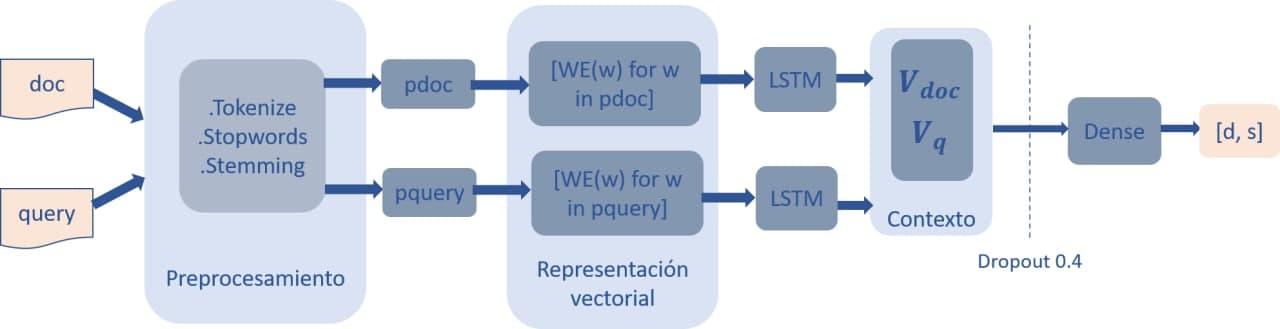
\includegraphics[width=\linewidth]{ ./images/lstm.jpg}
		\caption{Esquema del modelo neuronal con redes LSTM.}
		\label{lstm}
	\end{center}
\end{figure}

El proceso de \textit{tuning} de los hyperparametros del modelos se hizo de forma manual, usando una parte de los datos como conjunto de validación y la cantidad de épocas se seleccionó según el comportamiento que mostraban las curvas de entrenamiento.

\subsubsection{Evaluación.}

\subsection{Modelo Neuronal inspirado en MatchPyramid}

 En este último modelo decidimos explorar otras aproximaciones a la forma de determinar la similaridad semántica entre la consulta y un documento en particular. Para ello escogimos inspirarnos en modelo MatchPyramid \cite{193} que ha sido utilizado en tareas de \textit{text matching} y específicamente se ha estudiado su uso en recuperación de información \cite{194}. 
 
  En la Figura \ref{matchpyramid} se muestra la arquitectura del modelo propuesto. La entrada es procesada de igual manera a cómo fue explicado en la sección anterior.
  
La motivación detrás de MatchPyramid se basa en el éxito alcanzado por las CNN en el reconocimiento de imágenes dada su capacidad de abstraer patrones visuales. Por tanto propone resolver el problema de \textit{text matching} de una manera análoga al reconocimiento de imágenes. Para ello se hace uso de una matriz de \textit{matching} $M$ entre la consulta y el documento. Como se muestra en la Ecuación \ref{eq1} cada elemento $M{ij}$ va a representar la similaridad entre la palabra $w_i$ de la consulta y la palabra $w_j$ del documento, donde dicha similaridad va a estar dada por un operador $\otimes$ entre la repesentación vectorial de cada palabra, en este caso usaremos el producto. 

 \begin{equation}
 \label{eq1}
 M_{ij} = w_i \otimes w_j
 \end{equation} 
  
 La matriz $M$ construida sería lo que se considera la ''imagen'' y va a ser procesada por una capa convolucional con la que se pretende extraer diferentes niveles de patrones, seguido de una capa de \textit{pooling} con máximo como función de agregación para conservar solo los rasgos más significativos. A continuación se hace uso de la estrategia de dropout para combatir el overfitting del modelo. Por último se añade una capa densa que actúa como clasificador con función de activación softmax y que al igual que el otro modelo neuronal propuesto va a dar como salida el grado de similitud entre la consulta y el documento. 

\begin{figure}
	\begin{center}
		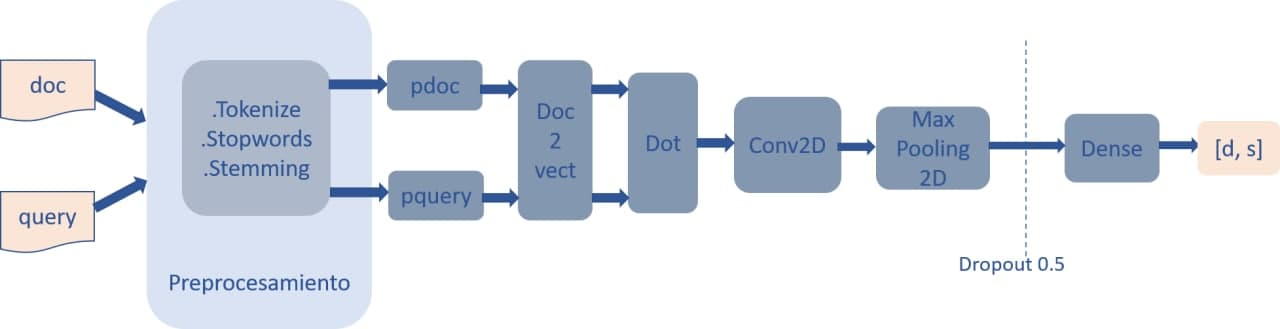
\includegraphics[width=\linewidth]{ ./images/match.jpg}
		\caption{Esquema del modelo neuronal inspirado en MatchPyramid.}
		\label{matchpyramid}
	\end{center}
\end{figure}

Al igual que para el modelo neuronal anterior el proceso de \textit{tuning} de los hyperparametros fue manualmente, tomando una parte de los datos como conjunto de validación y la cantidad de épocas se seleccionó acorde al comportamiento de las curvas de entrenamiento.

\subsubsection{Evaluación.}

\section{Expansión de Consultas}
El proceso de expansión de consultas es una técnica que tiene como objetivo enriquecer el contenido de la consulta con palabras adicionales, generalmente tomadas del vocabulario. Las palabras agregadas, llamados candidatos de expansión, se suponen que ayudan al proceso de matching del modelo a encontrar los documentos relevantes y resolver ambig\"uedades en consultas cortas. A pesar de no implementar esta variante de retroalimentación en el proyecto, consideramos importante reflejar el estudio realizado sobre las distintas alternativas existentes en el estado del arte, específicamente con la aplicación de word embeddings.  

Si se pretende emplear word embeddings para realizar este proceso, en lugar de realizar un \textit{matching} entre la consulta y el documento en el espacio latente, los vectores de palabras son usados para encontrar buenos candidatos para expandir la consulta. La selección de los mismos generalmente está basada en un vocabulario global, donde es usada una función de similaridad para obtener los términos correctos. Varios métodos [\cite{160}, \cite{190}, \cite{191}, \cite{165}] han sido propuestos para estimar la relevancia de los términos candidatos para la consulta. La mayoría de estos comparten un procedimiento: primero se realiza una comparación de las representaciones vectoriales de cada término candidato contra cada término de la consulta y es determinada una puntuación para cada uno de los candidatos. Luego son tomados los $k$ primeros términos y agregados al final de la consulta. Algunos modelos \cite{192} pueden adicionar métodos de filtrado, como la matriz de ocurrencia entre los términos candidatos y las palabras de la consulta. 

Por ejemplo en \cite{190} se proponen tres métodos que usan el embedding de cada término individual. A continuación se detallan brevemente:
\\

\textbf{Pre-retrieval kNN: } Dada una consulta $Q = [q_1, ..., q_m]$ se define el conjunto $C$ con los términos candidatos para la expansión donde $C = U_{q \in Q}(NN(q)) $ donde $NN(q)$ es el conjunto de los $k$ términos más cercanos a $q$ en el espacio de vectores de palabras empleado. Para cada término $t$ en $C$, se computa el promedio de la métrica del coseno entre $t$ y el resto de términos en $Q$. Luego, de acuerdo a esta puntuación son ordenados los términos en $C$ y los primeros $k$ son seleccionados como candidatos finales.
\\

\textbf{Post-retrieval kNN: } En esta aproximación emplean un conjunto de documentos pseudo-relevantes(PRD), o sea, aquellos documentos que estuvieron en los primeros lugares en respuesta a una consulta inicial. El objetivo es restringir el dominio de búsqueda de los términos candidatos. En lugar de buscar vecinos cercanos dentro de todo el vocabulario de la colección de documentos, se consideran solo aquellos términos que ocurren dentro de PRD. El resto del procedimiento es igual a la primera propuesta.
\\

\textbf{Pre-retrieval incremental kNN}
Esta propuesta es una extensión de \textit{pre-retrieval kNN}, variando la forma de calcular $NN(q)$, siendo ahora de forma incremental. Se realiza un proceso iterativo sobre la lista $NN(q)$ de los candidatos aportados por el término $q$ de la consulta. Sea $NN_l(q) = [t_1, t_2, ..., t_n]$ se consideran los primeros $k$ términos, o sea, $[t_1, t_2, ..., t_{n-k}]$. Luego se toma $t_1$ y se reordena la lista anterior con respecto a la similaridad con $t_1$. Este proceso continúa durante $l$ iteraciones.

\section{Recomendaciones}

Al analizar los desalentadores resultados obtenidos, proponemos para futuros trabajos realizar algunas modificaciones y utilizar otras herramientas.

\begin{enumerate}
	\item Las redes neuronales son muy sensibles a los hiperparámetros por lo que se considera interesante probar varios cambios en estos para alcanzar mejores resultados.
	\item Representar las sentencias mediante n-grams para obtener una encapsulación de entidades más completas, donde se tengan en cuenta las relaciones de posición entre términos.
	\item En el modelo MatchPyramid utilizar otros operadores en el cálculo de la matriz $M$.
	\item Implementar técnicas de retroalimentación como expansión de consultas. 
	\item Probar con otros corpus donde la cantidad de relaciones de relevancia no sea tan pequeña.
	\item Investigar sobre las ventajas que pudiéramos obtener con el uso del modelo Bidirectional Encoder Representations from Transformers(BERT) el cual tiene altas potencialidades capturando las características semánticas en un contexto.
\end{enumerate}
* 
* 
* 
* 
* 
* 

\section{Conclusiones}
 
 En este trabajo se realizó  el diseño, implementación, evaluación y análisis de un Sistema de Recuperación de Información, para el cual se proponen tres enfoques diferentes. Ninguna de las aproximaciones mostró resultados satisfactorios. Consideramos que uno de los factores que influyeron en el pobre desempeño de los modelos propustos fue la calidad de las colecciones con que se contó para los procesos de entrenamiento y evaluación. Estos conjuntos de datos presentanban un gran desequilibrio con respecto a la cantidad de parejas de consulta y documento que se consideraban similares y aquellas que no.
 
 A pesar de no haber obtenido los resultados deseados en cuanto al desempeño del Sistema de Recuperación de Información cabe destacar  la importancia de la investigación realizada, pues puede servir como punto de partida para tratar de lograr resultados mejores, por lo que para trabajos futuros recomendamos:

\begin{enumerate}
	\item Las redes neuronales son muy sensibles a los hiperparámetros por lo que se considera interesante probar varios cambios en estos para alcanzar mejores resultados.
	\item Representar las sentencias mediante n-grams para obtener una encapsulación de entidades más completas, donde se tengan en cuenta las relaciones de posición entre términos.
	\item En el modelo MatchPyramid utilizar otros operadores en el cálculo de la matriz $M$.
	\item Implementar técnicas de retroalimentación como expansión de consultas. 
	\item Probar con otros corpus donde la cantidad de relaciones de relevancia no sea tan pequeña.
	\item Investigar sobre las ventajas que pudiéramos obtener con el uso del modelo Bidirectional Encoder Representations from Transformers(BERT) el cual tiene altas potencialidades capturando las características semánticas en un contexto.
\end{enumerate}

%
% ---- Bibliography ----
%
\begin{thebibliography}{}
%
\bibitem{0} Jerey Pennington, Richard Socher, and Christopher D. Manning. 2014. Glove: Global vectors for word representation. In Empirical Methods in Natural Language Processing (EMNLP), pages 1532–1543.

\bibitem{1} Sanjeev Arora, Yingyu Liang, and Tengyu Ma. 2016. A simple but tough-to- beat baseline for sentence embeddings. Interna- tional Conference on Learning Representations.

\bibitem{2} Tomas Mikolov, Kai Chen, Greg Corrado, and Jeffrey Dean. 2013. Effi- cient estimation of word representations in vec- tor space. arXiv preprint arXiv:1301.3781.

\bibitem{3}Shengxian Wan, Yanyan Lan, Jiafeng Guo, Jun Xu, Liang Pang, and Xueqi Cheng. A deep architecture for semantic matching with multiple positional sentence representations. In Thirtieth AAAI Conference on Artificial Intelligence, 2016.

\bibitem{11} Jiafeng Guo, Yixing Fan, Liang Pang, Liu Yang, Qingyao Ai, Hamed Zamani, Chen Wu, W. Bruce Croft, and Xueqi Cheng. A deep look into neural ranking models for information retrieval. Information Processing and Management, page 102067, 2019.

\bibitem{12} Ryan Kiros, Yukun Zhu, Ruslan R Salakhutdinov, Richard Zemel, Raquel Urtasun, Antonio Torralba, and Sanja Fidler. Skip-thought vectors. In C. Cortes, N. D. Lawrence, D. D. Lee, M. Sugiyama, and R. Garnett, editors, Advances in Neural Information Processing Systems 28, pages 3294–3302. Curran Associates, Inc., 2015.

\bibitem{16} Po-Sen Huang, Xiaodong He, Jianfeng Gao, Li Deng, Alex Acero, and Larry Heck. Learning deep structured semantic models for web search using clickthrough data. In Proceedings of the 22nd ACM international conference on Information \& Knowledge Management, pages 2333–2338. ACM, 2013.

\bibitem{17} Baotian Hu, Zhengdong Lu, Hang Li, and Qingcai Chen. Convolutional neural network architectures for matching natural language sentences. In Advances in neural information processing systems, pages 2042–2050,


\bibitem{55}  Tomas Mikolov, Kai Chen, Greg Corrado, and Jeffrey Dean. Efficient estimation of word representations in vector space. arXiv preprint arXiv:1301.3781, 2013.

\bibitem{185} Yelong Shen, Xiaodong He, Jianfeng Gao, Li Deng, and Grégoire Mesnil. Learning semantic representations using convolutional neural networks for web search. In 23rd International Conference on World Wide Web’14,

\bibitem{178} Jiafeng Guo, Yixing Fan, Qingyao Ai, and W Bruce Croft. A deep relevance matching model for ad-hoc retrieval. In 25th ACM International Conf. CIKM’16, 2016.

\bibitem{205} Hang Li. Learning to rank for information retrieval and natural language processing. Synthesis Lectures on Human Language Technologies, 2011.

\bibitem{206} Sally Jo Cunningham, James Littin, and Ian H Witten. Applications of machine learning in information retrieval. 1997.

\bibitem{207} Tie-Yan Liu. Learning to rank for information retrieval. Springer Science \& Business Media, 2011.

\bibitem{208} Kevin Duh and Katrin Kirchhoff. Learning to rank with partially-labeled data. In Proceedings of the 31st annual international ACM SIGIR conference on Research and development in information retrieval, pages 251–258. ACM, 2008.

\bibitem{209} Zhe Cao, Tao Qin, Tie-Yan Liu, Ming-Feng Tsai, and Hang Li. Learning to rank: from pairwise approach to listwise approach. In Proceedings of the 24th international conference on Machine learning, pages 129–136. ACM, 2007

\bibitem{210} Christopher Burges, Tal Shaked, Erin Renshaw, Ari Lazier, Matt Deeds, Nicole Hamilton, and Gregory N Hullender. Learning to rank using gra- dient descent. In Proceedings of the 22nd International Conference on Machine learning (ICML-05), pages 89–96, 2005.

\bibitem{211} Wei Chen, Tie-Yan Liu, Yanyan Lan, Zhi-Ming Ma, and Hang Li. Ranking measures and loss functions in learning to rank. In Advances in Neural Information Processing Systems, pages 315–323, 2009.

\bibitem{237} Yelong Shen, Xiaodong He, Jianfeng Gao, Li Deng, and Grégoire Mesnil. A latent semantic model with convolutional-pooling structure for informa- tion retrieval. In Proceedings of the 23rd ACM international conference on conference on information and knowledge management, pages 101–110. ACM, 2014.

\bibitem{238} Aliaksei Severyn and Alessandro Moschitti. Learning to rank short text pairs with convolutional deep neural networks. In Proceedings of the 38th international ACM SIGIR conference on research and development in in- formation retrieval, pages 373–382. ACM, 2015.

\bibitem{241} Seonhoon Kim, Inho Kang, and Nojun Kwak. Semantic sentence matching with densely-connected recurrent and co-attentive information. In Proceedings of the AAAI Conference on Artificial Intelligence, volume 33, pages 6586–6593, 2019.

\bibitem{243} Sanjay Kamath, Brigitte Grau, and Yue Ma. Predicting and Integrating Expected Answer Types into a Simple Recurrent Neural Network Model for Answer Sentence Selection. In 20th International Conference on Computational Linguistics and Intelligent Text Processing, La Rochelle, France, April 2019. 

\bibitem{81}  Matthew E Peters, Mark Neumann, Mohit Iyyer, Matt Gardner, Christopher Clark, Kenton Lee, and Luke Zettlemoyer. Deep contextualized word representations. arXiv preprint arXiv:1802.05365, 2018. 

\bibitem{160} Fernando Diaz, Bhaskar Mitra, and Nick Craswell. Query expansion with locally-trained word embeddings. In Proceedings of the 54th Annual Meeting of the Association for Computational Linguistics (Volume 1: Long Papers), volume 1, pages 367–377, 2016.

\bibitem{165} Hamed Zamani and W. Bruce Croft. Estimating embedding vectors for queries. In Proceedings of the 2016 ACM International Conference on the Theory of Information Retrieval, ICTIR ’16, pages 123–132, New York, NY, USA, 2016. ACM.

\bibitem{190} Dwaipayan Roy, Debjyoti Paul, Mandar Mitra, and Utpal Garain. Using word embeddings for automatic query expansion. arXiv preprint arXiv:1606.07608, 2016.

\bibitem{191} Saar Kuzi, Anna Shtok, and Oren Kurland. Query expansion using word embeddings. In Proceedings of the 25th ACM international on conference on information and knowledge management, pages 1929–1932. ACM, 2016.

\bibitem{192} Navid Rekabsaz, Mihai Lupu, Allan Hanbury, and Hamed Zamani. Word embedding causes topic shifting; exploit global context! In Proceedings of the 40th International ACM SIGIR Conference on Research and Development in Information Retrieval, SIGIR ’17, pages 1105–1108, New York, NY, USA, 2017. ACM.

\bibitem{194} Pang, L., Y. Lan, J. Guo, J. Xu, and X. Cheng. 2016a. “A study of match pyramid models on ad-hoc retrieval”. arXiv preprint arXiv:1606.04648.

\bibitem{193} Pang, L., Y. Lan, J. Guo, J. Xu, S. Wan, and X. Cheng. 2016b. “Text Matching as Image Recognition”. In: Proc. AAAI.


\end{thebibliography}
\clearpage
%\addtocmark[2]{Author Index} % additional numbered TOC entry
%\renewcommand{\indexname}{Author Index}
%\printindex
\clearpage
%\addtocmark[2]{Subject Index} % additional numbered TOC entry
%\markboth{Subject Index}{Subject Index}
%\renewcommand{\indexname}{Subject Index}
%%                                                           clmomu01.ind
%-----------------------------------------------------------------------
% CLMoMu01 1.0: LaTeX style files for books
% Sample index file for User's guide
% (c) Springer-Verlag HD
%-----------------------------------------------------------------------
\begin{theindex}
\item Absorption\idxquad 327
\item Absorption of radiation \idxquad 289--292,\, 299,\,300
\item Actinides \idxquad 244
\item Aharonov-Bohm effect\idxquad 142--146
\item Angular momentum\idxquad 101--112
\subitem algebraic treatment\idxquad 391--396
\item Angular momentum addition\idxquad 185--193
\item Angular momentum commutation relations\idxquad 101
\item Angular momentum quantization\idxquad 9--10,\,104--106
\item Angular momentum states\idxquad 107,\,321,\,391--396
\item Antiquark\idxquad 83
\item $\alpha$-rays\idxquad 101--103
\item Atomic theory\idxquad 8--10,\,219--249,\,327
\item Average value\newline ({\it see also\/} Expectation value)
15--16,\,25,\,34,\,37,\,357
\indexspace
\item Baker-Hausdorff formula\idxquad 23
\item Balmer formula\idxquad 8
\item Balmer series\idxquad 125
\item Baryon\idxquad 220,\,224
\item Basis\idxquad 98
\item Basis system\idxquad 164,\,376
\item Bell inequality\idxquad 379--381,\,382
\item Bessel functions\idxquad 201,\,313,\,337
\subitem spherical\idxquad 304--306,\, 309,\, 313--314,\,322
\item Bound state\idxquad 73--74,\,78--79,\,116--118,\,202,\, 267,\,
273,\,306,\,348,\,351
\item Boundary conditions\idxquad 59,\, 70
\item Bra\idxquad 159
\item Breit-Wigner formula\idxquad 80,\,84,\,332
\item Brillouin-Wigner perturbation theory\idxquad 203
\indexspace
\item Cathode rays\idxquad 8
\item Causality\idxquad 357--359
\item Center-of-mass frame\idxquad 232,\,274,\,338
\item Central potential\idxquad 113--135,\,303--314
\item Centrifugal potential\idxquad 115--116,\,323
\item Characteristic function\idxquad 33
\item Clebsch-Gordan coefficients\idxquad 191--193
\item Cold emission\idxquad 88
\item Combination principle, Ritz's\idxquad 124
\item Commutation relations\idxquad 27,\,44,\,353,\,391
\item Commutator\idxquad 21--22,\,27,\,44,\,344
\item Compatibility of measurements\idxquad 99
\item Complete orthonormal set\idxquad 31,\,40,\,160,\,360
\item Complete orthonormal system, {\it see}\newline
Complete orthonormal set
\item Complete set of observables, {\it see\/} Complete
set of operators
\indexspace
\item Eigenfunction\idxquad 34,\,46,\,344--346
\subitem radial\idxquad 321
\subsubitem calculation\idxquad 322--324
\item EPR argument\idxquad 377--378
\item Exchange term\idxquad 228,\,231,\,237,\,241,\,268,\,272
\indexspace
\item $f$-sum rule\idxquad 302
\item Fermi energy\idxquad 223
\indexspace
\item H$^+_2$ molecule\idxquad 26
\item Half-life\idxquad 65
\item Holzwarth energies\idxquad 68
\end{theindex}

\end{document}
